\chapter{メッシュ地図を用いた自己位置推定}

\section{メッシュ地図での自己位置推定}
提案手法では, 自己位置推定の手法としてモンテカルロ自己位置推定\cite{MCL_paper}を用いた. モンテカルロ自己位置推定の数式などはAppendix \ref{app:monte_carlo}に示した. 提案手法における処理全体の流れとしてはAlg. \ref{alg:Overall}の通りである. このアルゴリズムの中で, (1)は\ref{sec:motion_update}節, (2)は\ref{sec:measurement_update}節, (3)は\ref{sec:estimate_current_pose}, (4)は\ref{sec:resampling}節でそれぞれ解説する.

\begin{algorithm}[htpb]
\SetAlgoLined
\caption{Semantic Mesh Localization Algorithm}
\label{alg:Overall}
 initialize particles $x_{0}$ and weights $w_{0}$\;
 \For{each time instance $t$}{
    acquire segmented image $y_{t}$\;
    motion update (1) \;
    \For{number of particles}{
        project 3D mesh map to 2D image in the view of particle $i$ as image $f_{t}^{i}$ \;
    }
    measurement update (2) \;
    normalize weights $w_{t}$\;
    estimate current pose $x_{t}$ (3)\;
    \If{resampling is needed}{
        resampling (4) \;
    }
 }
\end{algorithm}

%%%%ここからはコメントアウト
\begin{comment}
自己位置推定は最初の姿勢$x_{0}$,これまでの姿勢制御値$u_{1},u_{2}, ... ,u_{t}$, これまでのセンサ値のリスト$z_{1},z_{2}, ... ,z_{t}$からエージェントが現在の姿勢を更新する問題である. 自己位置推定を確率的な問題と扱うために現在の真の姿勢$x^{*}_{t}$に関する条件付き確率密度関数
\begin{equation}
    p_{t}(x|x_{0},u_{1},u_{2}, ... ,u_{t},z_{1},z_{2}, ... ,z_{t})
\end{equation}
を考える. $u_{1},u_{2}, ... ,u_{t}$を$u_{1:t}$, $z_{1},z_{2}, ... ,z_{t}$を$z_{1:t}$とおくと,
\begin{equation}
    p_{t}(x|x_{0}u_{1:t},z_{1:t})
\end{equation}
と表記できる. また, $u_{t}$を制御指令値と表記したがオドメトリやIMUなどのセンサを使った結果生じる移動量とすることもでき, ロボティクスにおいてはむしろそれが一般的である\cite[p108]{ueda_prob_robotics}. また移動量$u_{t}$については何らかの要因によって誤差が入っている時がある. 今回の実験では\ref{sec:dataset}節のとおり, 真値の移動量にガウス分布に従う誤差を加えた.\par 自己位置推定は時刻$t$における信念分布
\begin{equation}\label{eq:believe_total}
    b(t)=p_{t}(x|x_{0}u_{1:t},z_{1:t})
\end{equation}
を求めることに帰結する. \ref{eq:believe_total}をさらに分解すると入力である$x_{0},u_{1:t},z_{1:t}$, 状態遷移モデル$x_{t} \sim p(x|x_{t-1},u_{t})$, 観測モデル$z_{t} \sim p(z|x_{t})$に分解できる.\par 状態遷移モデル$x_{t} \sim p(x|x_{t-1},u_{t})$は信念分布$\hat{b}_{t}$として
\begin{equation}\label{eq:motion_update}
    \hat{b}(t)=p_{t}(x|x_{0},u_{1:t},z_{1:t-1})=p_{t}(x|x_{0},u_{1:t})
\end{equation}
と表現できる. $b_{t}$との違いはまだセンサ値$z_{t}$が反映されていない点である.この部分の詳細は\ref{sec:motion_update}節で詳しく述べる.\par 信念分布$b_{t}$は式\ref{eq:motion_update}の$\hat{b}_{t}$に\ref{sec:measurement_update}節で述べる観測モデルからの値$p(z_{t}|x)$を反映させることでできる. 式としては
\begin{equation}\label{eq:believe_equal}
    b_{t}(x)=\hat{b}_{t}(x|z_{t})=\frac{p(z_{t}|x)\hat{b}_{t}(x)}{p(z_{t})}=\eta p(z_{t}|x)\hat{b}_{t}(x)
\end{equation}
となる.
\end{comment}
%%%ここまでコメントアウト


\subsection{事前分布の更新}\label{sec:motion_update}
パーティクルフィルタにおいて事前分布の更新の目的は, 誤差を含むオドメトリやIMUなどの移動量に対してある確率分布に従ってパーティクルを分散させて信念分布$\hat{b}_{t}$の分布内に真の位置$x_{t}^{*}$をカバーすることである. パーティクル$i$において, 時刻$t-1$におけるパーティクルの位置$x_{t-1}^i$及び誤差を含む移動量$\Delta x_{t}$に対して事前分布の更新後の位置$\hat{x}_{t}^i$は
\begin{equation}\label{eq:motion_update_chapter}
    \hat{x}_{t}^i = x_{t-1}^i + \Delta x_{t} + \delta
\end{equation}
と表される. 今回の実験において, 式\ref{eq:motion_update_chapter}における$\delta$は平均$0$分散$\sigma^{2}$に従う正規分布$\mathcal{N}(0,\sigma^{2})$からドローできる.
\begin{equation}
    \delta \sim \mathcal{N}(0,\sigma^{2})
\end{equation}

\subsection{事後分布の更新}\label{sec:measurement_update}
パーティクルフィルタにおける事後分布の更新の目的は時刻$t$におけるパーティクルの尤度$w^{i}_{t}$を算出して後述する自己位置推定結果の算出やリサンプリングに役立てることである. \par セグメンテーションされたがカメラ画像を$y_{t}$パーティクルの位置$\hat{x}_{t}^{i}$から見た三次元メッシュ地図を二次元のRGB画像に変換したものを$f_{t}^{i}$として, 2つの画像を比較してセマンティックなクラスが一致したピクセルのみ抽出した画像を$d_{t}^{i}$とする. パーティクル$i$の尤度$w_{t}^{i}$は
\begin{equation}\label{eq:particle_likelihood}
    w_{t}^{i} = p(d_{t}^{i}|f_{t}^{i},y_{t},\hat{x}_{t}^{i},\mathcal{M})
\end{equation}
と表される. 式中の$\mathcal{M}$は三次元メッシュ地図を表している. \par 尤度算出のアルゴリズムはAlg. \ref{alg:calc_likelihood}の通りである. また, アルゴリズム中のsemantic scoreはピクセルのクラスごとに割り振られた値を出力する関数である. クラスごとの出力値は\ref{sec:env_appendix}節の表\ref{tab:likelihood_parameter}にある.

\begin{algorithm}[htpb]
 get segmented image as $y_{t}$ \;
 get mesh map image as $f_{t}^{i}$ \;
 $w^{i}_{t}$ = 0.0\;
 \If{The sizes of the $y_{t}$ and $f_{t}^{i}$ images match}{
    \For{$j=0$; $j<$size of image's height}{
        \For{$i=0$; $i<$size of image's width}{
            mesh class = semantic class of image $y_{t}$ at coordinate (i,j) \;
            image class = semantic class of image $f_{t}^{i}$ at coordinate(i,j) \;
            \If{mesh class == image class}{
                $w^{i}_{t}$ = $w^{i}_{t}$ + semantic score(image class) \;
            }
        }
    }
 }
 \Return $w^{i}_{t}$\;
 
 \caption{Calculating Likelihood Algorithms}
 \label{alg:calc_likelihood}
\end{algorithm}


\subsection{自己位置推定の結果の出力}\label{sec:estimate_current_pose}
\ref{sec:measurement_update}節において算出したパーティクル$w^{i}_{t}$を尤度が高い順に並べ替えて, 表\ref{tab:MCL_parameter}のAveragemumberの値$n$から上位$n$個のパーティクルのXYZ座標の平均を位置$x_{t}$のXYZ座標とした. 角度について, 本手法ではクオータニオンを角度表現に使っているが, クオータニオンは平均値の算出の計算が煩雑であるため\cite{Quaternion_average}最も尤度の高いパーティクルのクオータニオンを位置$x_{t}$の角度とした.

\subsection{リサンプリング}\label{sec:resampling}
 提案手法において用いられたリサンプリングの手法は系統サンプリング\cite{systematic_resampling_review}\cite{madow1944}と呼ばれるものである. パーティクル数を$n$, 各パーティクル$i$の尤度を$w_{t}^{i}$, 全パーティクルの尤度の合計を$\mathcal{W}$とすると系統サンプリングのアルゴリズムはAlg. \ref{alg:systematic_resampling_algorithm}の通りである.

\begin{algorithm}[htpb]
$w$ = empty vector\;
$acc = 0$\;
\For{$i=0$; $i<n$}{
    $acc = acc + w_{t}^{i}$\;
    $w$.append($acc$)\;
}
$step=\mathcal{W}/n$\;
$r \sim \mathcal{U}(0,step)$\;
$curpos=0$\;
$nw$ = empty vector\;
\While{size of $nw$ $<$ $\mathcal{W}$}{
    \eIf{$r<w[curpos]$}{
        $nw$.append($w_{t}^{curpos}$)\;
        $r=r+step$\;
        \If{$r>\mathcal{W}$}{
            $r=r-\mathcal{W}$\;
            $curpos=0$\;
        }
    }
    {
        $curpos+=1$\;
    }
}

\Return $nw$\;

 \caption{Systematic Resampling Algorithm}
 \label{alg:systematic_resampling_algorithm}
\end{algorithm}

%% Bonnetの解説
\section{セグメンテーション手法}
提案手法の有用性を示すための実験において, カメラ画像のセマンティックセグメンテーションの手法はBonnet\cite{milioto2019icra}を使用した. BonnetはGithub上で公開されているオープンソースのフレームワークであり, ROS環境下でリアルタイムなセグメンテーションをすることができるのが大きな特徴である. また, BonnetはGithub\cite{Bonnet_Github}から訓練済みのモデルをダウンロードすることが可能であり, CityScapes, Synthia\cite{RosCVPR16}, Persons\cite{Persons_Link}, Crop-Weed(CWC)\cite{chebrolu2017ijrr}の4つのデータセットから条件に応じた訓練済みデータを入手できる. 今回の実験ではCityScapesから学習した訓練済みデータを使用した.

\begin{figure}[htbp]
\begin{center}
\begin{tabular}{c}
\begin{minipage}{1.0\hsize}
\begin{center}
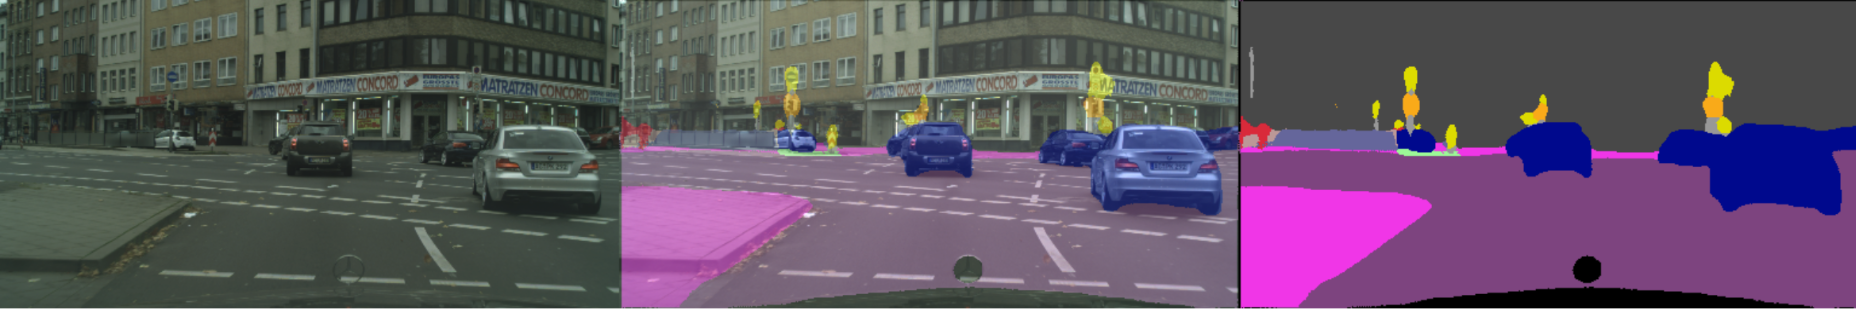
\includegraphics[width=14cm]{./picture/semantic_segmentation_bonnet.png}
\caption{Bonnetによるセマンティックセグメンテーション}
\label{fig:Bonnet}
\end{center}
\end{minipage}
\end{tabular}
\end{center}
\end{figure}

% Vexel Gridで点を間引いた間隔とかSLAMのやり方について書く
\section{メッシュ地図生成}
メッシュ地図のもととなる三次元点群地図の生成はデータセットのGround Truthを位置データを使用して行われた. そこからPCLのVoXelGrid Filter\cite{PCL_VexelGrid_Link}\cite{VoxelGrid_paper_1}\cite{VoxelGrid_paper_2}の機能を用いてクラスごとに異なる間隔で点群の間引きを行った.  メッシュ地図の生成は三次元点群地図からPCLのGreedyTriangulation\cite{Marton09ICRA}の機能を用いて作成した. 上記の通りの作成された点群地図は図\ref{fig:Point_Cloud_Map}, メッシュ地図は図\ref{fig:Mesh_Map}の通りである.

\begin{figure}[htbp]
\begin{center}
\begin{tabular}{c}
\begin{minipage}{1.0\hsize}
\begin{center}
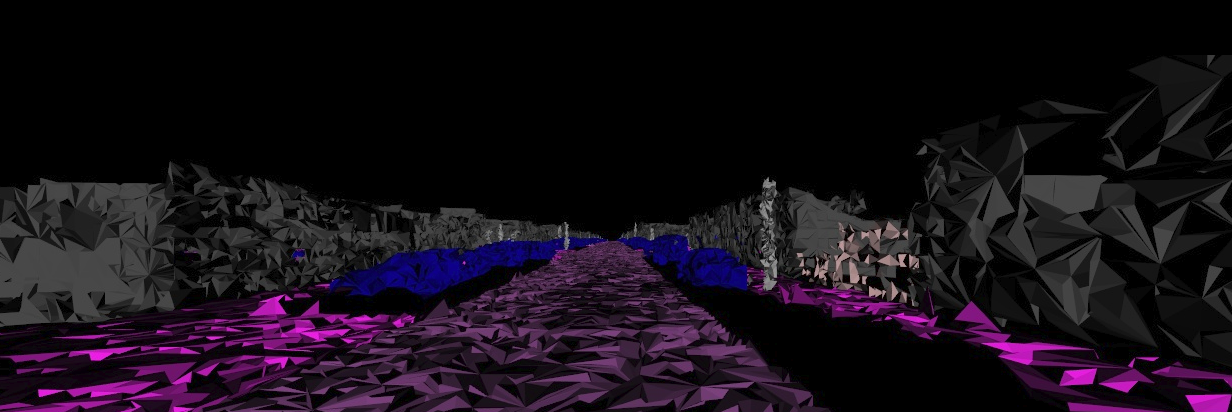
\includegraphics[width=14.5cm]{./picture/mesh_map.png}
\caption{メッシュ地図}
\label{fig:Mesh_Map}
\end{center}
\end{minipage}
\end{tabular}
\end{center}
\end{figure}

%\subsection{補足}